\begin{figure*}[t]
\centering
\footnotesize
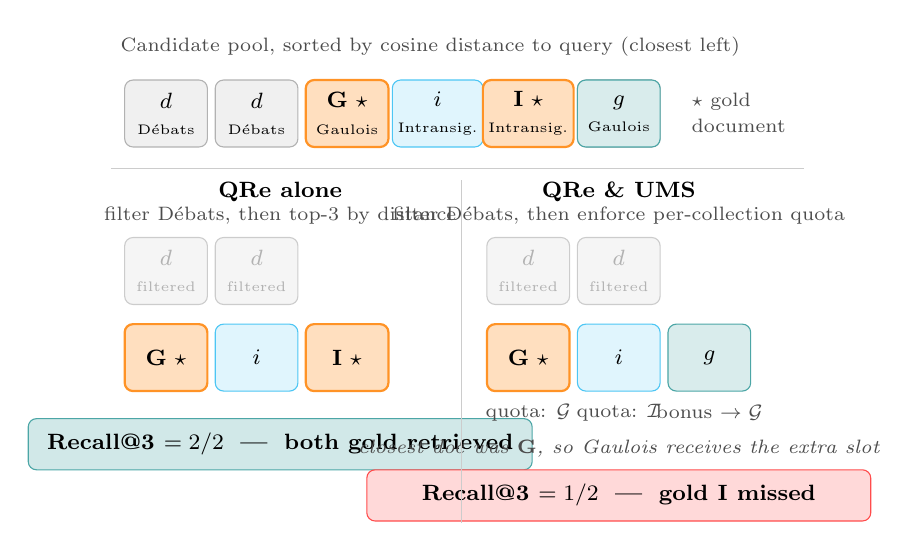
\begin{tikzpicture}[
  doc/.style={
    rectangle, rounded corners=3pt, draw, line width=0.4pt,
    minimum width=1.05cm, minimum height=0.85cm,
    align=center, inner sep=2pt, font=\footnotesize
  },
  debats/.style={doc, fill=gray!12, draw=gray!60},
  gaulois/.style={doc, fill=teal!15, draw=teal!70},
  intran/.style={doc, fill=cyan!12, draw=cyan!70},
  gold/.style={doc, fill=orange!25, draw=orange!85, line width=0.8pt},
  filtered/.style={doc, fill=gray!8, draw=gray!40, text=gray!60},
  result/.style={
    rectangle, rounded corners=3pt, draw, line width=0.4pt,
    minimum width=6.4cm, minimum height=0.65cm, align=center,
    font=\footnotesize\bfseries, inner sep=3pt
  },
  goodres/.style={result, fill=teal!18, draw=teal!70},
  badres/.style={result, fill=red!15, draw=red!70},
  caption/.style={font=\scriptsize, text=black!70},
  divider/.style={draw=black!20, line width=0.3pt}
]

% --- Pool header ---
\node[caption, anchor=west] at (-0.2, 4.7)
  {Candidate pool, sorted by cosine distance to query (closest left)};

% --- Pool: 6 documents in distance order ---
\node[debats]  (p1) at (0.5, 3.85) {$d$ \\ \tiny Débats};
\node[debats]  (p2) at (1.65, 3.85) {$d$ \\ \tiny Débats};
\node[gold]    (p3) at (2.8, 3.85) {$\mathbf{G}\ \star$ \\ \tiny Gaulois};
\node[intran]  (p4) at (3.95, 3.85) {$i$ \\ \tiny Intransig.};
\node[gold]    (p5) at (5.1, 3.85) {$\mathbf{I}\ \star$ \\ \tiny Intransig.};
\node[debats]  (p6) at (6.25, 3.85) {$g$ \\ \tiny Gaulois};

\node[caption, anchor=west] at (7.05, 4.0) {$\star$ gold};
\node[caption, anchor=west] at (7.05, 3.7) {document};

% Repaint p6 as gaulois (was wrong style above — overwrite to keep code linear)
\node[gaulois] at (6.25, 3.85) {$g$ \\ \tiny Gaulois};

% --- Divider ---
\draw[divider] (-0.2, 3.15) -- (8.6, 3.15);

% =========================================================
% LEFT PANEL: QRe alone
% =========================================================
\node[font=\footnotesize\bfseries] at (1.95, 2.85) {QRe alone};
\node[caption] at (1.95, 2.55) {filter Débats, then top-3 by distance};

% Filtered (greyed out)
\node[filtered] (q1) at (0.5, 1.85) {$d$ \\ \tiny filtered};
\node[filtered] (q2) at (1.65, 1.85) {$d$ \\ \tiny filtered};

% Selected (3 gold-style or teal background to mark "kept")
\node[gold]   (q3) at (0.5, 0.75) {$\mathbf{G}\ \star$};
\node[intran] (q4) at (1.65, 0.75) {$i$};
\node[gold]   (q5) at (2.8, 0.75) {$\mathbf{I}\ \star$};

\node[goodres] at (1.95, -0.35) {Recall@3 $= 2/2$ \;\textemdash\; both gold retrieved};

% =========================================================
% RIGHT PANEL: QRe & UMS
% =========================================================
\node[font=\footnotesize\bfseries] at (6.25, 2.85) {QRe \& UMS};
\node[caption] at (6.25, 2.55) {filter Débats, then enforce per-collection quota};

% Filtered
\node[filtered] (r1) at (5.1, 1.85) {$d$ \\ \tiny filtered};
\node[filtered] (r2) at (6.25, 1.85) {$d$ \\ \tiny filtered};

% Selected
\node[gold]    (r3) at (5.1, 0.75) {$\mathbf{G}\ \star$};
\node[intran]  (r4) at (6.25, 0.75) {$i$};
\node[gaulois] (r5) at (7.4, 0.75) {$g$};

% Quota labels
\node[caption] at (5.1, 0.05) {quota: $\mathcal{G}$};
\node[caption] at (6.25, 0.05) {quota: $\mathcal{I}$};
\node[caption] at (7.4, 0.05) {bonus $\rightarrow \mathcal{G}$};

\node[caption, font=\scriptsize\itshape] at (6.25, -0.4)
  {closest doc was $\mathbf{G}$, so Gaulois receives the extra slot};

\node[badres] at (6.25, -1.0) {Recall@3 $= 1/2$ \;\textemdash\; gold $\mathbf{I}$ missed};

% Vertical separator between panels
\draw[divider] (4.25, 3.0) -- (4.25, -1.35);

\end{tikzpicture}
\caption{Worked example illustrating the marginal cost of uniform allocation
on cross-newspaper questions.
The candidate pool (top) contains six documents from the three collections
($d$: \textit{Les Débats}, $g$: \textit{Le Gaulois}, $i$: \textit{L'Intransigeant}),
ordered by cosine distance to the query. Bold uppercase symbols ($\mathbf{G}$, $\mathbf{I}$)
mark the two gold documents.
\textbf{Left:} QRe filters out \textit{Les Débats} and returns the top-3
remaining candidates, retrieving both gold documents.
\textbf{Right:} QRe \& UMS applies the same source filter but then enforces the
uniform quota: one mandatory slot per active collection plus a bonus slot for
the collection whose closest document is globally nearest the query
(\textit{Le Gaulois} here). The bonus slot promotes the trailing $g$ over
the gold $\mathbf{I}$, which is therefore missed.}
\label{fig:qre-ums-tradeoff}
\end{figure*}